\chapter{Collaboratively generating hypotheses}
\begin{figure}[h] 
  \centering
  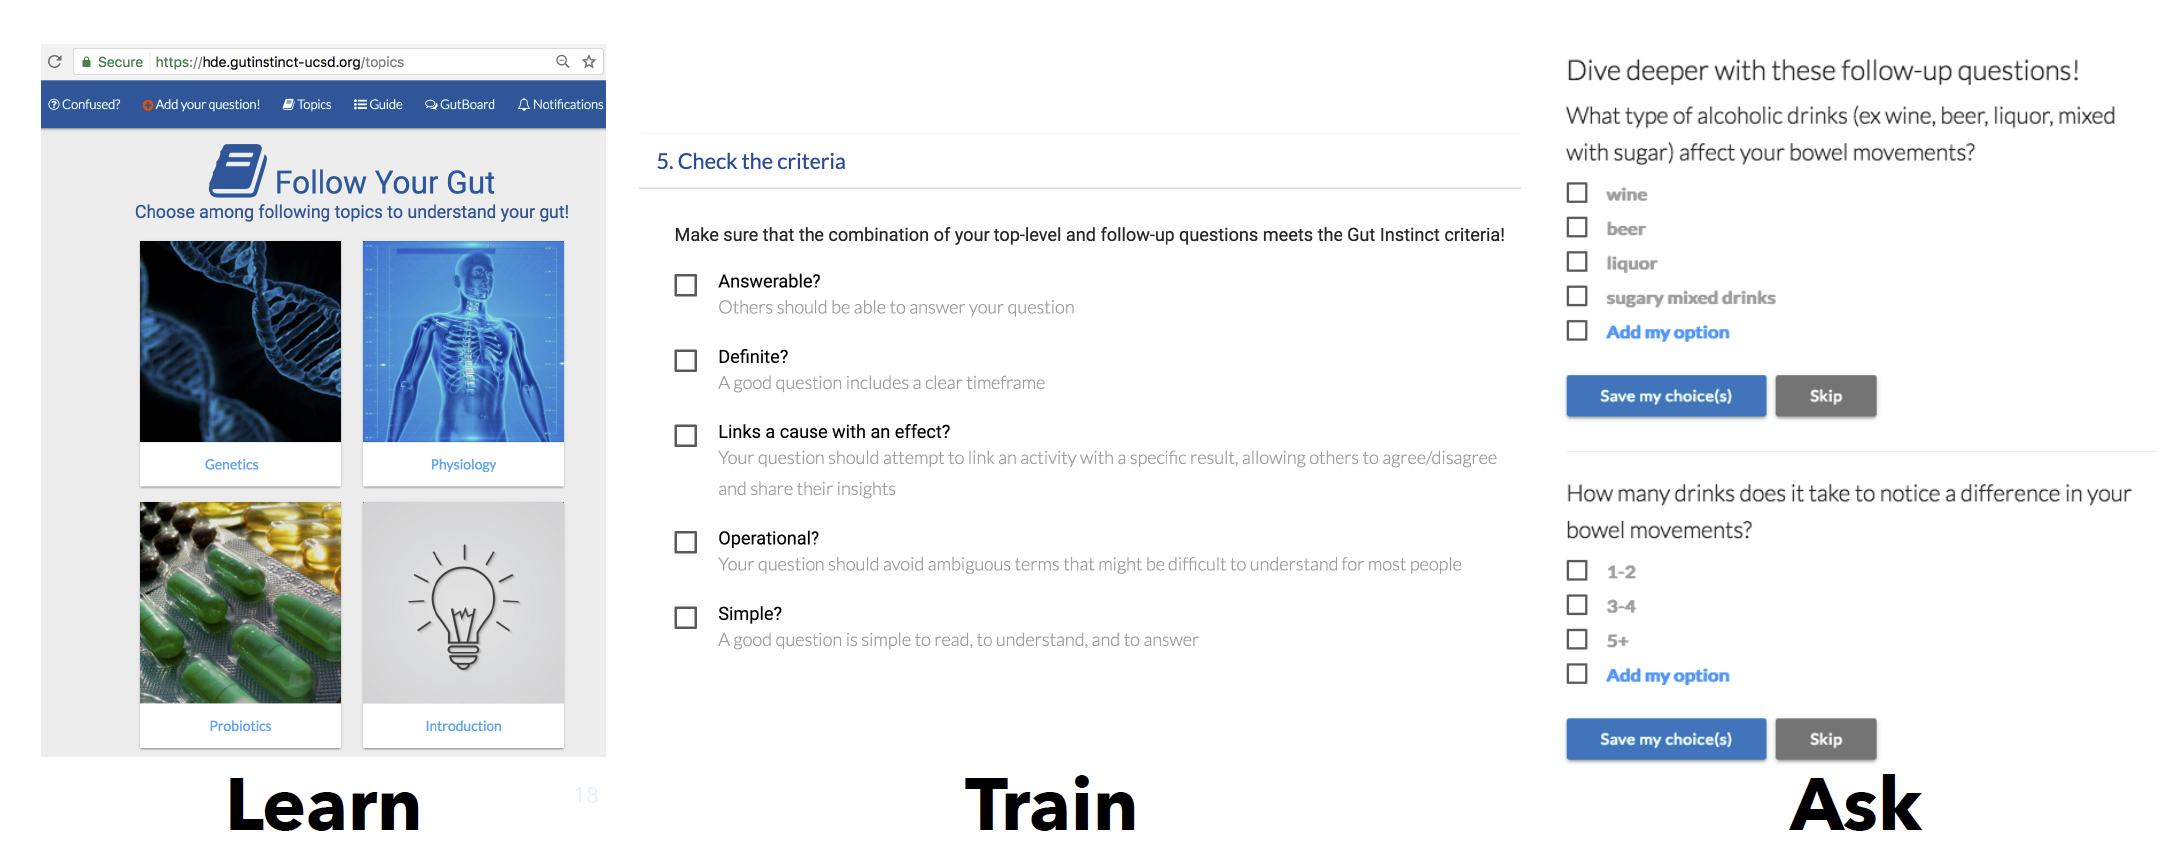
\includegraphics[width=1.0\textwidth]{figures/docent/fig-0.png}
  \caption[The Docent Learn-Train-Ask workflow]
{The Docent Learn-Train-Ask workflow.\index{docent-0}}
  \label{fig:docent-0}
\end{figure}

\textit{People’s lived experiences provide intuitions about health.
Can they transform these personal intuitions into testable hypotheses
that could inform both science and their lives? This
paper introduces an online learning architecture and provides
system principles for people to brainstorm causal scientific
theories. We describe the Learn-Train-Ask workflow that
guides participants through learning domain-specific content,
process training to frame their intuitions as hypotheses,
and collaborating with anonymous peers to brainstorm related
questions. 344 voluntary online participants from 27
countries created 399 personally-relevant questions about the
human microbiome over 4 months, 75 (19\%) of which microbiome
experts found potentially scientifically novel. Participants
with access to process training generated
hypotheses of better quality. Access to learning materials improved
the questions’ microbiome-specific knowledge.
These results highlight the promise of performing personally 
meaningful scientific work using massive online learning
systems}

%%%%%%%%%%%%%
Thinking like a scientist involves generating useful questions,
operationalizing them as hypotheses, and testing them
with experiments. While people generate (implicit) intuitions
from lived experiences, transforming tacit knowledge into
explicit questions is not easy. People don’t always realize the
extent of their knowledge and even when they do, asking questions 
that can be answered by others to yield clear, actionable
insights is hard. For instance, people often bury
questions in long entries (Figure~\ref{fig:docent_1}. Transforming intuitions
into falsifiable questions is a key skill for scientists and designers
alike. How can people create questions that are novel
(contain new information), useful (relate to and potentially
extend existing scientific knowledge), easy to answer, and
specific (relate to only one topic)? Such questions can
potentially accelerate research in nascent scientific domains,
such as the human microbiome.

This paper contributes (1) the Learn-Train-Ask method for
people to perform personally meaningful scientific work by
sharing personal insights and receiving feedback from
others, and (2) its embodiment in Docent — a novel
crowdsourcing system for causal scientific questions. Docent
enables novices to ask useful questions by learning domainspecific
content, undergoing process training to develop
task-specific skills, and collaborating with online peers. A
between-subjects study evaluated this new method by measuring
the quality of participants’ questions to test causal scientific
theories about the human microbiome. 344 voluntary
online participants from 27 countries — including participants
from the American Gut Project, Open Humans,
Coursera, and Reddit — signed up to share personally-relevant
questions about the human microbiome. Participants
created 399 questions, 75 (19\%) of which microbiome experts
found novel. Participants with access to process training
generated hypotheses of better quality. Access to
learning materials improved the questions’ microbiome-specific
knowledge. These results highlight the promise of performing
personally-meaningful scientific work using
massive online learning systems.


%\begin{figure}[h] 
%  \centering
%  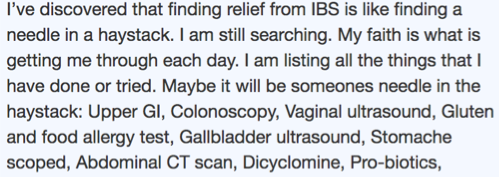
\includegraphics[width=1.0\textwidth]{figures/docent/fig-1.png}
%  \caption[]
%{This post to a Mayo Clinic forum shows how people
%seeking advice online combine many ideas into one post..\index{docent-1}}
%  \label{fig:docent-1}
%\end{figure}

\begin{wrapfigure}{r}{0.5\textwidth}
  \centering
  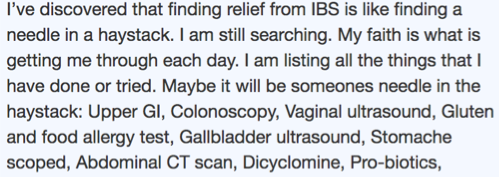
\includegraphics[width=0.5\textwidth]{figures/docent/fig-1.png}
  \caption[Post to a Mayo Clinic forum]
{This post to a Mayo Clinic forum shows how people
seeking advice online combine many ideas into one post..\index{docent-1}}
  \label{fig:docent-1}
\end{wrapfigure}

%%%%%%%%%%%%%%%%%%%%%%%%%%%%%%%%%%%%%%%%%%%%%%%%%%%%%%%%%%%%%
\section{The Docent Social Computing System}
The Docent social computing system enables people to create specific, personal hypotheses by providing: content learning \& process training; a guided question-asking interface; and an online collaboration platform. Docent was designed via multiple iterations of early pilot studies. Docent’s pilot participants were ~50 lead users of the American Gut Project \& Health Data Exploration workshop (hdexplore.calit2.net). Early participants used the website to provide in-person feedback about the interface. As the sys-tem matured, later participants provided both explicit online \& in-person feedback along with usage data that led to a number of improvements. For instance, a pilot session led to the idea to enable editing others’ questions to improve clarity (especially for non-native English speakers).

The Docent web application is built with Meteor (meteor.com), and extends Gut Instinct~\cite{Pandey2017} that also leverages learning materials, but does not address causal theory generation. The front-end uses BlazeJS (blazejs.org) and is styled with Materialize (materialize.css).

\subsection{Learn-Train-Ask: From Intuitions to Hypotheses}
Docent embodies three main principles. The first is two-way integration of learning and asking questions for improved conceptual understanding of the microbiome. Novel, domain-specific work (such as asking questions for micro-biome discovery) needs to integrate a novel idea with existing knowledge, perhaps even using specific terms/metrics in the process (e.g. Bristol stool scale for quality of bowel movement). To forge a two-way link between learning and asking questions, Docent provides online lectures and feed-back on the questions people create using scientific material. For instance, for a question about the effects of probiotics on mood among people suffering from gastrointestinal diseases, Docent would provide feedback using lectures about probiotics, gastrointestinal diseases, and the gut-brain axis.
The two attributes that training questions seek to model are a) that others can answer them, and b) that each addresses a single topic. Training helps participants get a feel for how precise questions should be: overly vague and overly specific terms both reduce a question’s utility. To link many ideas with one cause, a sequence of questions can iteratively refine a hypothesis space. For instance, a question linking probiotics use to bowel movements might begin by asking how frequently people consume probiotics and in which form, following up by asking about bowel movements.
Third, Docent provides clear success criteria: creating useful questions. Docent converts question-asking and answering into an engaging social interaction by enabling people to participate in multiple ways, such as by asking questions, adding follow-ups, editing questions to improve clarity, or responding to questions. A new user can access the entire Docent system only after adding a question.

\begin{wrapfigure}{r}{0.5\textwidth}
  \centering
  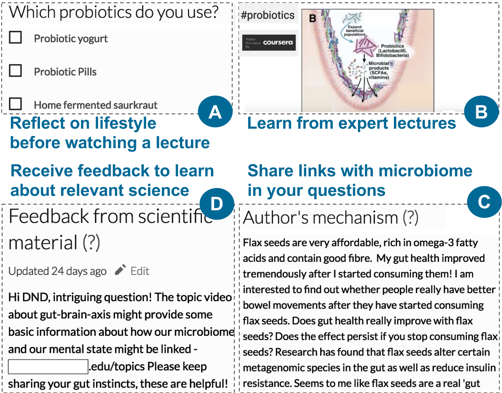
\includegraphics[width=0.5\textwidth]{figures/docent/fig-2.png}
  \caption[User flow of Docent learning module]
{User flow of Docent learning module. Participants reflect on their lifestyle by (A) answering a personal question before (B) watching an online lecture about probiotics and the microbiome. Participants (C) must propose a mechanism when adding a question and (D) they receive feedback from scientific material on their questions. Probiotics was one of 16 topics for which Docent provided ~5min long expert lectures.\index{docent-2}}
  \label{fig:docent-2}
\end{wrapfigure}
 
\subsection{Learn content: Integrate Concepts with Insights}
Docent’s learn module teaches people about the gut microbiome using online lectures, lifestyle questions, feedback from scientific material on questions, and guessing potential mechanisms (Figure~\ref{fig:docent-2}). We describe each below. 

%\begin{figure}[h] 
%  \centering
%  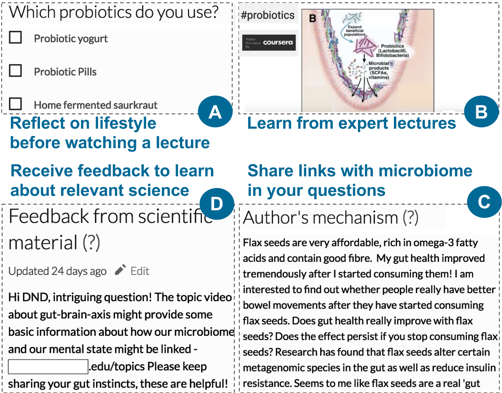
\includegraphics[width=1.0\textwidth]{figures/docent/fig-2.png}
%  \caption[User flow of Docent learning module]
%{User flow of Docent learning module. Participants reflect on their lifestyle by (A) answering a personal question before (B) watching an online lecture about probiotics and the microbiome. Participants (C) must propose a mechanism when adding a question and (D) they receive feedback from scientific material on their questions. Probiotics was one of 16 topics for which Docent provided ~5min long expert lectures.\index{docent-2}}
%  \label{fig:docent-2}
%\end{figure}

Online lectures to improve conceptual understanding: The human microbiome is nascent, yet fast-growing. There is a lot of room for new contributions, but few people have up-to-date and accurate knowledge, even to the extent that it exists. People ask more questions when the learning material causes inconsistencies in their understanding of a topic~\cite{Miyake1979a}. Since few people know about the microbiome, Docent uses introductory learning material curated from Gut Check, a Coursera MOOC ~\cite{Knight2016}, rather than scientific papers that may be too abstruse. Apart from introductory material about the microbiome, Docent also provides learning material about specialized topics, such as gastrointestinal diseases \& the gut-brain axis, to engage people in guided discovery learning based on their interests and health conditions (Figure~\ref{fig:docent-2}B).

 Personal questions to improve reflection: Prompting participants to explicitly reflect on the learning topic can increase curiosity and question-quality~\cite{Aleven2006, Law2016}. Before watching a lecture about the microbiome, Docent invites people to answer questions that make them reflect on the connection between the learning material and their lifestyle (Figure~\ref{fig:docent-2}A).

Guessing a mechanism to reflect on question and knowledge: Docent asks people to guess mechanistic explanations for how the microbiome can play a role in answering their questions (Figure~\ref{fig:docent-2}C). This is intended to help users learn by connecting personal observations with existing knowledge~\cite{Simon2004}.

Feedback from scientific material: Rapid, relevant feedback improves quality~\cite{Hattie2007}. The first author provided links to scientific papers and web content in response to people’s questions. To integrate questions with Docent’s learning material, they also received feedback on their questions using links to the Coursera MOOC lecture hosted on Docent (Figure~\ref{fig:docent-2}D). Participants also added scientific papers to questions. 

\subsection{Process training: From Intuitions to Scientific Questions}
Docent uses three components to help people ask useful questions: a training guide, expert examples, and a question-asking checklist (Figure~\ref{fig:docent-3}). 

\begin{figure}[b] 
  \centering
  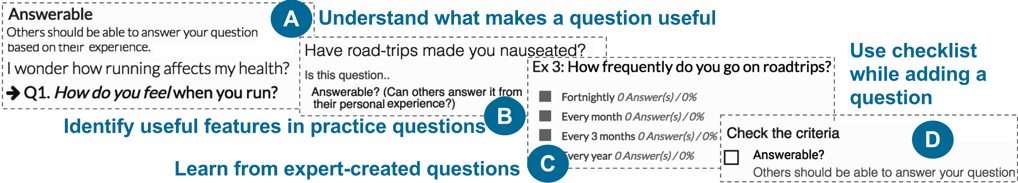
\includegraphics[width=1.0\textwidth]{figures/docent/fig-3.png}
  \caption[The Docent training process]
{The Docent training process. People (A) learn what makes a question useful, (B) practice on sample questions, and (C) read expert-curated questions. (D) When asking a question, a checklist reminds people to ensure their question meets the criteria for useful questions. Answerability was one of 5 features for which Docent provided training.\index{docent-3}}
  \label{fig:docent-3}
\end{figure}

Training guide to identify useful features: New Docent participants must add a question before accessing the entire system (learning, training, and the GutBoard). Before asking a second question, however, a user needs to complete the training guide: people learn about five features of successful questions; train by identifying these features in two sample questions (Figure~\ref{fig:docent-3}A,B); and then immediately ask a question. Training draws on successful techniques from crowd work and peer assessment by using gold standards~\cite{Kittur2013} and rubrics~\cite{Andrade2005}. When adding a question, a checklist reminds participants about the features of good questions (Figure~\ref{fig:docent-3}D).

\subsection{Ask well-framed questions }
Good questions specify a cause and associated effects.

\textit{Two-step question format to separate cause and effect}: Docent questions comprise two parts: a top-level question identifies a cause (e.g., frequency of consuming probiotics). A follow-up question links the cause to a specific insight from the user (e.g., effects of consuming probiotics). The creator can add multiple follow-ups to link a cause to many effects.

\textit{Templated options to reduce common errors}: Poor and/or vague options can discourage responses, erode esprit de corps, and model bad behavior that others follow. To counter this, Docent provides popular templated multiple-choice options. These templates are editable, but providing templates helps people be specific.

\textit{Cues to improve question quality}: These cues comprise alert messages when people add long or short options; notes about details needed in their questions; and restricting people from adding a question without providing a potential mechanism or comment.

\subsection{GutBoard: Crowd responses, Discussion, Expert feedback}
The GutBoard is designed for quick question traversal, easy response, and collaboration. Only the top-level question from each question is displayed: if a user is not interested in, say probiotics, they can simply skip that set. However, to access follow-ups, people need to answer the top-level question by selecting from the existing options or adding their own. To focus people’s attention on specific questions, the first author starred promising questions that people can access from the Starred tab (Figure~\ref{fig:docent-4}). Starring signifies that a question is likely of high quality or broad interest, and helps focus participants’ answering efforts on them. Docent also enables people to bookmark questions of interest, so they can visit them again. 

To de-incentivize lurking and increase engagement, the GutBoard shows only one question at a time; we call this sequential access. When people could see multiple questions simultaneously (parallel access), they skimmed through many questions without interacting with them. 

\begin{wrapfigure}{r}{0.5\textwidth}
  \centering
  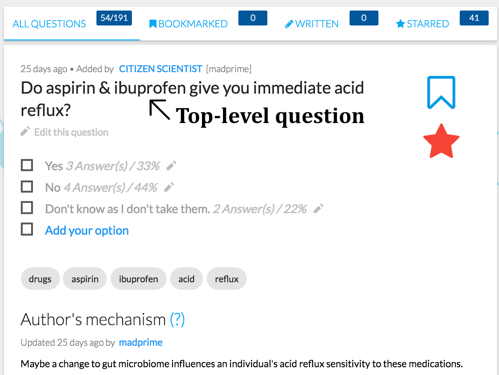
\includegraphics[width=0.5\textwidth]{figures/docent/fig-4.png}
  \caption[Participants can see follow-up questions, add new options, new follow-up questions, edit the question, guess potential mechanisms, and bookmark]
{After answering a top-level question, participants can see follow-up questions, add new options, new follow-up questions, edit the question, guess potential mechanisms, and bookmark. A star (added by an expert) shows that this question may be promising for further enquiry by people.\index{docent-4}}
  \label{fig:docent-4}
\end{wrapfigure}

%%%%%%%%%%%%%%%%%%%%%%%%%%%%%%%%%%%%%%
\section{Hypotheses: Effect of Learning and Training on Question Quality}
Learn-Train-Ask scaffolds collaborative scientific question generation. We tested the following hypotheses in the context of brainstorming potential causal relationships in the human gut microbiome.

\textbf{H1. Access to learning improves question’s content.}
While people’s questions are based on their experiences and curiosity, aligning them with what is already known about the microbiome can uncover novel insights. Alternately, learning can make people reflect less on their personal knowledge and more on institutional knowledge, reducing the novelty of their questions. A question is deemed to have good content if it is insightful (exhibits microbiome-specific knowledge) and novel (contains potentially new knowledge for microbiome science).

\textbf{H2. Just-in-time training improves question’s structure.}
We hypothesize that training helps people create useful questions for receiving feedback as well as for generating insights for researchers. A question is deemed to have good structure if it is easy for other participants to answer and focuses on one topic.

\section{Study: Scaffolds for Better Questions}
A between-subjects study compared the participants’ question quality across four conditions: Learn, Train, Neither and Both. In the Learn condition, participants saw online lectures, answered personal questions, guessed mechanisms, and received feedback from scientific material on their questions (provided by the first author). The Train condition provided participants access to a training guide, expert examples, and checklist. In the Neither condition, participants did not have access to either the Learn or Train step, while in the Both condition they had access to both. All participants had access to the question-asking and GutBoard collaboration module (with required condition-appropriate adjustments — e.g., participants in Learn and Both conditions were asked to guess the mechanism for their question, while participants in the other two conditions were asked to add a discussion comment). The GutBoard content was unique to the participants for a specific condition, to ensure that participants were not influenced by behavior in other conditions. 

\subsection{Method}
Participants were randomly assigned to one of the four conditions. Each gave participants access to a condition-specific Docent. Each condition began with an introductory tour describing the significance of microbiome research and the importance of their contributions towards making discoveries. At the end of the tour, participants in every condition had to add one question (using identical question-asking modules) before moving on. Docent sent regular email reminders about site activity. 

\subsection{Participants}
Recruitment: Participants were recruited via online publicity. To invite people especially interested in their microbiome, the American Gut Project emailed 550 participants. Docent was promoted on the American Gut Project’s and their collaborators’ Facebook and Twitter pages. Docent was added as a project on Open Humans (openhumans.org) — a platform where people donate their personal data for scientific research and participate in scientific experiments. Docent was posted on multiple subreddits pertaining to health and lifestyle (e.g., reddit.com/r/keto) and added as an optional assignment to the Gut Check Coursera MOOC~\cite{Knight2016}. Participation was voluntary and unpaid; participants were entered in a raffle for an American Gut Microbiome kit (provided for \$99 on American Gut’s crowdfunding page (fundrazr.com/campaigns/4Tqx5)) on survey completion.

\subsection{Measures}
Dependent variables comprised structure, content, and creativity of questions (Table 1). American Gut researchers with multiple years of post-PhD expertise independently rated all 399 questions. (330 questions were rated by three; 69 were rated by two). The average ICC measure for 3 raters was 0.48 with 95\% CI[0.42,0.54], (F (328,656) = 3.73, p<.001). Raters agreed that evaluating novelty was difficult since the nascent microbiome literature is rapidly growing.

Raters were instructed to assign points for structure if it asked participants about a specific topic that they could answer. For example, “How often do you consume fermented foods?” was rated as both answerable by participants and specific, while, “Does our modern agricultural system affect our microbiome?” was neither answerable nor specific. Question content was the sum of insightfulness and novelty. Insightfulness addressed the quality of the microbiome content in the questions. Novelty was assessed as the potential to create new knowledge in the microbiome field and operationalized as the lack of research papers about the specific question. For example, “Does consuming bone broth improve digestion?” was rated as both insightful and novel, while, “Can microbiome cure cancer?” was neither insightful nor novel. Broad questions related to well-studied topics or those fishing for links with the microbiome, such as the difference between generic vegetarian and meat-based diet were not deemed novel. A question was considered creative if it suggested an interesting idea without necessarily drawing it from personal experience. 

\subsection{Results}
344 participants completed the baseline exercise, continuing to the condition-specific intervention (Learn, Train, Both, or Neither). Participants who asked follow-on questions were scored as described above; those who did not were scored as 0. Table 2 shows, for each condition, the total number of participants, the number that provided questions, the total question points, and the average score across all participants. The overall quality of the questions generated in the combined Train+Learn condition is the highest (0.56 points) and appears to stand out from the others. We used a permutation test (a kind of bootstrapping method) to assess the statistical reliability of this apparent interaction, namely, whether the combined Learn-Train condition produces better questions than is expected from the independent main effects of the Learn and Train conditions. Indeed, a permutation test with 10,000 replications found that the observed differences in question points are different than the expected differences (generated by the main-effect marginals) as they fall outside the 95\% confidence interval [-24.5, 24.5], p <.05. The three score components (structure, content, and creativity) were pairwise weakly correlated (r=0.32, p < 0.02; r=0.19, p < 0.17; r=0.33, p < 0.01). 

\begin{figure}[h] 
  \centering
  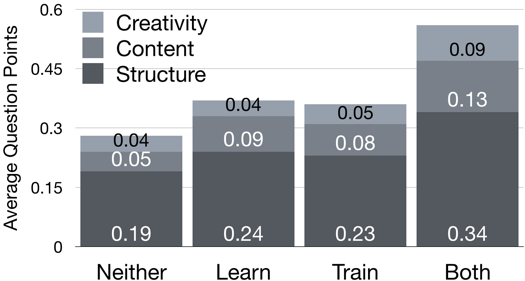
\includegraphics[width=1.0\textwidth]{figures/docent/fig-5.png}
  \caption[Training improved the overall question quality but learning did not]
{Training improved the overall question quality (p <.05) but learning did not (p $<$ 0.1). H1: Training marginally improved question structure (p <.06). H2: Learning improved question content (p <.05).\index{docent-5}}
  \label{fig:docent-5}
\end{figure}

\textit{Total question points}: Training improved overall question quality (M=0.31, vs. M=0.47); a permutation test with 10,000 replications found that the observed difference in question points are different than the expected differences as they fell outside the 95\% CI[-19.5, 19.5], p <.05. Learning did not improve overall question quality (M=0.32, vs. M=0.46); a permutation test with 10,000 replications found that the observed differences in question points are not different than the expected differences as they did not fall outside the 95\% CI[-29.5, 29.5], p < 0.1. (Figure~\ref{fig:docent-5})

\textit{Structure}: H1: Did access to training material (Train and Both conditions) improve the structure of questions relative to not having access (Learn and Neither conditions)? Training marginally improved question structure (M=0.21, vs. M=0.29); a permutation test with 10,000 replications found that the observed difference in question structure points are different than the expected differences as they did not fall outside the 95\% CI[-9.5, 9.5], p <.06.

\textit{Content}: H2: Did learning material (Learn and Both conditions) improve the content of questions relative to not having access (Train and Neither conditions)? Learning improved question content (M=0.06, vs. M=0.11); a permutation test with 10,000 replications found that the observed difference in question content points fell outside the 95\% CI[-9, 9], p <.05.

\textit{Creativity}: Did training or learning material (Learn and Both conditions) impact the creativity score of questions relative to not having access (Train and Neither conditions)? Neither training (M=0.04 vs. M=0.07; 10,000-replication permutation test 95\% CI[-4, 4], p < 0.08) nor learning (M=0.05 vs. M=0.07; 10,000-replication permutation test 95\% CI[-4, 4], p < 0.2) improved the creativity score.

%%%%%%%%%%%%%%%%%%%%%%%%%%%%%%%
\section{Discussion}
\subsection{The effect of learning and training on questions}
As a check of random assignment, participants’ required pre-intervention question was of comparable quality in all conditions. Participants in the Both condition scored higher total question points after the intervention. Training en-forced a tutorial when asking a question, and the add-question module presented heuristics for asking better ques-tions. This tight integration may have enabled people to focus their questions on a specific topic and frame their questions to be answerable by others. Moreover, the pres-ence of learning material might have provided a useful setup and improved participant engagement leading to greater number of questions, and question points.

The study found a significant effect for learning on content ratings and a marginally significant effect for training on structure ratings. This asymmetry could be substantive: that learning improves content, but training only lightly improves structure. Alternatively, it could be a statistical mi-rage: the lower inter-rater reliability for content might show an effect if there isn’t one. Inter-rater reliability was higher for structure (M=0.65; 95\% CI[0.59,0.69] (F (328,656) = 6.59, p < .001)) than content (M = 0.11; 95\% CI[0.04,0.18], (F (328,656) = 1.37, p <.001)).
We hypothesize that content learning more clearly helped because domain knowledge provided insights and, potentially, ideas for questions, whereas the benefits for training heuristics were less clear. Some participants mentioned that understanding the learning material deeply wasn’t their goal, which is corroborated by our experience designing and building the notes feature. Pilot feedback led us to create a time-annotated collaborative notes section alongside lecture videos. People could add notes about the lectures, raise clarifying questions with specific points in the video and answer others’ questions. Collaborative, time-annotated notes below lecture videos have shown to improve social interaction and learning~\cite{Lee2015}. However, people hardly used the notes features. After limited uptake, we removed these notes.

Participants watched 2.5 of 15 lectures on average. Moreover, in the Both condition, the combination of training and learning materials might have provided both useful content and sufficient structure for novices to utilize well. These results suggest that citizen scientists improve their work when presented with specific, just-in-time training. Self-guided question improvement may be valuable more broadly, as poor questions and question bloat are common problems in many social computing systems~\cite{Yang:2014:ARQ:2631775.2631809}.

\subsection{Which topics did the questions deal with?}
The best questions had three features: they shared a clear insight from the participants’ life (frequently elaborated upon in the discussion section of the question), enabled others to answer them from their lifestyle, and linked to known microbiome research (Table 3). Common question themes included probiotics; fermented foods; the consumption of fruits and vegetables in different forms; medicine usage; activities like exercises; stool quality \& consistency. The three most popular lectures viewed discussed diet, antibiotics, and probiotics, hinting that either people were inspired by the lectures or at the very least, the lectures may have satisfied some of participants’ curiosity about the links between their lifestyle and the microbiome. 50\% of participants with learning mentioned that the lectures influenced their questions.
Personal health was a big motivator; 78\% of questions pertained to diseases (e.g., Irritable Bowel Syndrome), general health and well-being (obesity) or medication. 90\% of survey respondents were motivated by personal health to ask questions. People created questions that linked activities with observable results (e.g., evacuation of bowel before colonoscopy with frequency of bowel movements after the procedure), but also raised questions that were driven more by curiosity about the microbiome: these questions inquired about their American Gut results, or the effect of a certain lifestyle choice (e.g., fasting) on microbiome, or microbiome’s effect on health (e.g., anxiety). 37\% of all questions contained “hypotheses” i.e. they identified relationships between clearly identified variables (e.g., “Does eating probiotic foods reduce sugar cravings?”), while 46\% only contained curiosity about the microbiome (e.g., “Hydrocolonic therapy change gut microbiome?” [sic]). Some of these questions were difficult even for experts to answer, since they are topics of active research (e.g., brain-gut axis~\cite{Mayer15490}).

\subsection{How novel are the questions?}
75 of the 399 questions were found to be novel by the American Gut Project researchers. Novelty was defined as “Is there a chance the world will learn something?” The probiotic-sugar question above is novel because no published work addresses it directly. Other work on the sugar-microbiome relationship establishes plausibility~\cite{Haukioja2008}. Such questions meet Docent’s primary objective: to uncover insights about topics where people’s lived experiences provide them more knowledge than lab experts. Docent-like citizen science platforms can leverage people’s lived experience to identify novel questions that experts have missed out and to evaluate these questions.

\begin{figure}[t] 
  \centering
  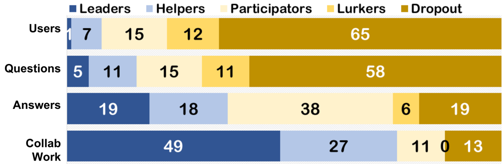
\includegraphics[width=1.0\textwidth]{figures/docent/fig-6.png}
  \caption[Distribution of role types]
{Distribution of role types for the 68 participants in the Both condition who added at least one question. The Leader formed 1\% of participants but contributed 19\% of the answers and 49\% of all collaborative activity (adding follow-ups, editing others’ question, adding options). Dropouts formed 65\% of participants and added one question each (57\% of all questions) but contributed to only 13\% of collaborative work. .\index{docent-6}}
  \label{fig:docent-6}
\end{figure}

\subsection{Emergent behavior, Engagement, and Growth}
Docent offers more avenues for active collaboration than traditional web fora. People can create questions, answer and edit questions, create follow-ups, and guess potential mechanisms. Participants added a total of 2424 answers, 74 follow-up questions, 466 new options and 358 mechanism/ discussion comments. Discussion comments fell into three types, sorted by popularity: (a) sharing personal insights; (b) sharing potential mechanisms for the question; and (c) providing links to related online resources. People edited others’ questions 119 times. Most edits were done by leaders and collaborators who attempted to clarify the question. None of the edits were reverted by the authors hinting that the edits were acceptable to them. Different ways to contribute creates different informal roles and behavior patterns in social computing systems, from leaders who perform all the activities to lurkers who may watch but not actively engage in collaborative activities (Table 4). Figure~\ref{fig:docent-6} shows the work distribution by roles in the Both condition.

Prior citizen science platforms have demonstrated lurker and dabbler behavior~\cite{Eveleigh2014}. Since people perform work on citizen science platforms, they require a prominent “circuit of engagement” [38]. Systems research comprises many choices; some we evaluate, others follow from prior work, \& some are hunches. To counter lurker behavior, Docent employs three techniques: First, Docent encourages members’ self-selection using a strategy that hides Docent’s content (lectures, training, and the GutBoard) until people add one question. Making even small contributions makes people feel more vested in the effort as a part of a community and removes their fear of performing a novel activity~\cite{Resnick2011}. Extending these ideas can be useful for future work. Second, the GutBoard’s continuous question updates provides social translucence~\cite{Resnick2011}. Third, Docent sends regular email and social media updates to engage the community.

\subsubsection{From Asking Questions to Building a Community}
Docent’s 20 email templates cover three areas: 1) user-activity specific e.g., reminder when someone added a follow-up question to a user’s question; 2) condition-specific e.g., weekly emails about activity on the platform for the user’s condition; 3) general reminders e.g., creating a username, or adding a question if participants had not done so already. Activity emails were sent each time a user’s question received an edit, follow-up question, option, discussion comment, or when experts starred the question. Docent sent weekly general updates and links to tutorials.
 
A renowned microbiome expert recorded answers to popular questions which were subsequently mailed to participants and uploaded on social media channels. Docent maintained an active profile on Facebook and Twitter (240 and 224 followers respectively) by providing updates about platform activity, researchers’ feedback on people’s questions, and microbiome-relevant scientific articles and studies. Despite attempts to engage people, Docent saw high dropouts. Of 1630 participants, 907 (55\%) took up usernames; and 344 participants (21\%) added at least one question.

\subsubsection{Two Optimizations Significantly Improve Scaling}
To efficiently handle hundreds of participants, Docent initially renders only the first two questions while the remaining questions are rendered in the background. Docent also reduces page load times by storing markers in the browser’s local storage for frequently accessed details, e.g., last-seen question. This enables Docent to fetch and show the next question on subsequent login rather than having to pull all questions and then traverse to the last-seen question. 

\subsection{Future Work: Diversity \& Social Behavior}
Of the 344 participants who added a question, 219, who provided location information, hailed from 27 countries. 174 participants (80\%) were from US or UK who asked 76\% of questions. This is not without reason —Docent’s online publicity was focused on the American Gut Project and its offshoot the British Gut Project. However, people in these countries may have higher socio-economic, educational, and technological status than the average global (or even, national) citizen (80\% of our survey respondents had at least an undergraduate degree; an American Gut Project kit costs \$99). MOOCs face a similar challenge: educated and affluent learners complete online classes at higher rates~\cite{Kizilcec2017b}. Science and humanity will likely benefit from diverse global participants~\cite{Henrich2010a}, as in Lab in the Wild~\cite{Reinecke2015}.

Diversity brings another design challenge. Diverse participants interpret prompts like Likert scale differently. People might also use terms that are not obvious to others. For instance, one participant asked about the frequency of “hoovering your home” which likely was lost on some participants. Since Docent participants hail from dozens of countries, terms need to be understood broadly. Participants could potentially flag such questions for clarification. 

\textit{Willingness to share private information}: Only 6\% of survey respondents said they did not feel comfortable sharing personal insights. This is promising; however, there were questions that some may feel embarrassed to answer — e.g., questions pertaining to bowel movements, flatulence, and sexual activity. For these cases, questions and options can be rephrased — e.g., “Do you suffer from bouts of flatulence?” can be changed to “In the past week, how often have you suffered from flatulence?” enabling people to provide some useful information rather than entirely avoiding such questions. Moreover, specific communities’ motivation can be focused on generating specific insights~\cite{Chandler2013}. Docent already has many questions raised by participants suffering from different ailments; such patient groups may have specific insights as well as greater motivation to share them in exploratory projects~\cite{Karkar2017a}.

\textit{Different strokes for different folks}: Docent users were volunteers. Multiple survey respondents mentioned that busyness impeded their platform usage. We hypothesize that encouraging moderators may increase platform stickiness. We plan to create guides and have people try different roles which can boost creative thinking~\cite{Teevan:2017:BWC:3059454.3059467}. With a diverse participant set — health-hackers, MOOC learners, even some advanced microbiome students — people’s attention can be put to specific tasks that they want to contribute to. For instance, MOOC learners may be more interested in unearthing mechanisms for people’s hypotheses. Such differentiated roles, including different levels of editor, have contributed to the success of social computing systems like Wikipedia~\cite{Krieger2009}.

\textit{Validating hypotheses shared by participants}: One early benefit of our work is that American Gut researchers are using the best Docent questions to potentially add/revise the metadata catalogue in the American Gut Project. Moreover, with the right online support, citizens can design and run experiments to test some of the hypotheses (e.g. probiotics reduces sugar cravings). Scaling causal reasoning could transform many domains. One interested party is the non-profit Open Humans platform where people volunteer their personal data (e.g., microbiome/genomic data) and provide access to researchers to use their data.

%%%%%%%%%%%%%%%%
\section{Conclusion}
This paper investigated integrating learning and training with online scientific work. Experts rated 75 of 399 questions as potentially scientifically novel. Participants with access to process training generated hypotheses of better quality. Access to learning materials improved the questions’ microbiome-specific knowledge.  The Learn-Train-Ask method can be applied towards next steps in the scientific process, namely designing and running experiments. This study also illustrates the challenges of designing a social computing system that engages voluntary participants in performing personally-relevant scientific work. Such online experiences also naturally provide a problem-based learning setup for better learner engagement. Intui-tions gathered from a large online crowd can significantly scale up scientific inquiry by augmenting scientific expertise with insights and know-how drawn from the lived experiences of diverse individual people. We believe that dual-objective online systems that combine learning with personally meaningful work can enable people to meet their needs.


